
\chapter{Control de Agentes Basados en Planificaci\'on Continua} \label{pagcap3}

La problem\'atica abordada por Moya en \cite{gbraun:tesisMarioMoya}, \cite{moya08:_planif_contin_como_contr_de_agent_robot},
\cite{moya08:_un_planif_contin_concur_para_agent_robot} y \cite{moya09:_agent_delib_basad_en_contin}
es la planificaci\'on en ambientes din\'amicos y no determin\'isticos. 
El objetivo principal es la implementaci\'on de un agente de prop\'osito general
que pueda operar en dominios del mundo real lidiando con m\'ultiples
eventos y con otros agentes.

El trabajo presenta un framework para la implementaci\'on de 
agentes deliberativos cuyo ra\-zo\-na\-mien\-to est\'a basado en planificaci\'on
continua. La implementaci\'on est\'a \'integramente desarrollada en
Ciao Prolog \cite{ciao-reference-manual-tr}.
Lo novedoso de este tipo de planificadores es que est\'an aptos para ambientes
reales permitiendo al agente persistir indefinidamente
en su entorno, es decir, que no se detiene al alcanzar una meta
sino que la ejecuci\'on contin\'ua mediante la formulaci\'on de nuevas
metas. De esta manera, el agente contin\'ua planificando y actuando. 
Algunos experimentos con esta implementaci\'on fueron realizados bajo el
dominio del F\'utbol de Robots,
utilizando Rakiduam. Rakiduam es un equipo de f\'utbol de robots
con licencia GNU\footnote{\emph{General Public License}.} 
que ha participado en numerosas ediciones
del Campeonato Argentino de F\'utbol con Robots (CAFR) con resultados m\'as que
satisfactorios. Algunos de ellos fueron publicados en \cite{kogan07:_rakid},
\cite{kogan06:_aspec_de_y_de_del} y \cite{trevisani09:_rakid}.

En el presente cap\'itulo se estudia con m\'as profundidad
esta implementaci\'on. En la secci\'on \ref{cap3:desProblema}
se hace un breve repaso del problema planteado por Moya. 
En la secci\'on \ref{cap3:caracter\'isticas} se detallan
las caracter\'isticas del Framework y el Planificador
Continuo que implementa. Por \'ultimo, en la secci\'on
\ref{cap3:intregracion}, se explica
la integraci\'on del traductor PDDL con el presente
framework basado en planificaci\'on continua.



\section{Descripci\'on del Problema} \label{cap3:desProblema}


La {\bf planificaci\'on continua} est\'a orientada a resolver problemas
en ambientes din\'amicos, por lo tanto, se encarga de atacar
problemas del mundo real. Este m\'etodo de planificaci\'on es denominado
``cl\'asico'', es decir, que no tiene separadas las etapas de 
planificaci\'on y ejecuci\'on sino, que se encuentra planificando
de manera continua en el tiempo. Hasta el momento de la
publicaci\'on de este framework, la planificaci\'on continua solamente
hab\'ia sido presentada en forma conceptual en \cite{russell03:_artif_intel}.
	
La tem\'atica que aborda el trabajo de Moya es el desarrollo de 
una arquitectura para agentes que soporte tanto \emph{control
reactivo} como \emph{deliberativo} y, en consecuecia, permitir que el agente
pueda actuar de manera competente y efectiva en un ambiente real.
En \cite{hanks90:_issues_in_archit_for_plann_and_execut}, Hanks y Firby, 
sugieren tratar de alcanzar un sutil
equilibrio entre estas dos estrategias: \emph{deliberaci\'on}
y \emph{reacci\'on}. La primera estrategia implica tomar todas las decisiones
factibles en forma tan anticipada en el tiempo como sea posible.
Mientras que la segunda, consiste en demorar las decisiones
que se tomen actuando, \'unicamente, en el \'ultimo momento posible.

Un agente que pueda pensar a futuro ser\'a capaz de considerar m\'as
opciones y, por lo tanto, estar\'a m\'as informado para decidir
qu\'e acci\'on tomar. Sin embargo, debido a que la informaci\'on
sobre el futuro puede ser poco confiable y, en muchas
situaciones del mundo real, dif\'icil o incluso imposible de obtener,
puede ser razonable tambi\'en actuar a \'ultimo momento.

En resumen, esta implementaci\'on aborda los problemas planteados
previamente dotando a un agente inteligente con 
capacidades deliberativas y reactivas, brindando as\'i,
la posibilidad de elegir cu\'al ser\'ia la mejor forma de
actuar frente a un problema determinado.  



\section{Caracter\'isticas Principales del Framework} \label{cap3:caracter\'isticas}

Tal como comentamos arriba, el dise\~{n}o del agente tiene
dos modos de operaci\'on: reactivo y deliberativo. Por simplificaci\'on,
el trabajo profundiza sobre el modo deliberativo y la posibilidad
de escoger en qu\'e modo actuar.

La implementaci\'on prove\'e un subsistema de control que interact\'ua directamente
con los sensores y efectores de un agente. El sistema recibe las percepciones
y devuelva acciones que pueden ser provistas tanto por el modo
reactivo como por el modo deliberativo.
Desde el punto de vista modular, la organizaci\'on sigue
los principios del modelo BDI (Belief, Desire, 
Intention) \cite{gbraun:rao91a}. 

Una de las caracter\'isticas principales, en la implementaci\'on, 
es el uso de hilos\footnote{En Ingl\'es, \emph{threads}.}.
El framework mantiene dos hilos principales de ejecuci\'on,
uno para el controlador, que toma nuevas percepciones
y actualiza el estado del agente, y otro para el planificador,
que intentar\'a encontrar el plan que satisfaga las metas y
percepciones actuales.
Estos hilos son definidos en Ciao Prolog usando
\emph{data predicates}. Los \emph{data predicates}
est\'an compuestos exclusivamente
por hechos que pueden ser observados, agregados o eliminados
din\'amicamente.

La arquitectura modular del framework se muestra
a continuaci\'on. 


	\begin{figure}[h!]
                \centering
		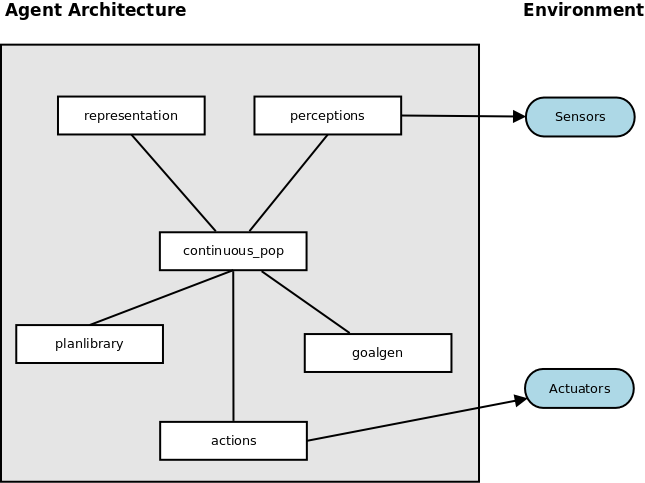
\includegraphics[width=9cm,height=8cm]{arq_modular.png}
		\caption{Arquitectura Modular del Framework de
                  Planificaci\'on Continua}
		\label{framework:modules}
	\end{figure}



	\subsection{Algoritmo de Planificaci\'on Continua}
	
	El algoritmo de planificaci\'on continua, presentado en \cite{gbraun:tesisMarioMoya}, es un
	bucle que obtiene percepciones, actualiza el estado actual 
	e intenta generar un plan.
	
	Una extensi\'on importante de la implementaci\'on es la capacidad
	de elegir un plan predefinido de una librer\'ia de planes. Por lo 
	tanto, cuando el planificador es invocado, recibe un plan inicial
	de la librer\'ia de planes. En caso que no se encuentre un plan
	acorde, se comienza con uno vac\'io.
	
	El algoritmo tiene tres estados bien definidos:
	
	\begin{itemize}
	
	\item En primer lugar, reformula las metas
	luego de procesar los deseos del agente. Entonces, se
	remueven enlaces no soportados y as\'i se evitan acciones
	con precondiciones falsas debido a cambios en los deseos
	del agente. A continuaci\'on, el algoritmo elimina acciones 
	redundantes que ya no son necesarias en el plan. Esta eliminaci\'on de 
	acciones conlleva un reemplazo de enlaces causales\footnote{Un enlace causal 
	es de la forma $A \longrightarrow^{p} B$ donde $A$ y $B$ son acciones 
	y $p$ es una proposici\'on 
	que es precondici\'on de la acci\'on $B$. La ejecuci\'on de $A$ 
	hace verdadero a $p$ para $B$ \cite{russell03:_artif_intel}.}. 
	
	\item El siguiente paso es una conducta heredada del Planificador
	de Orden Parcial (POP) \cite{gbraun:pop:1991}. Tal conducta involucra resolver 
	precondiciones abiertas. Para esto, se selecciona una precondici\'on
	e intenta resolverse agregando una nueva acci\'on o utilizando una
	ya existente.
	
	\item El \'ultimo paso del algoritmo es verificar si se ha alcanzado
	el conjunto actual de metas, es decir, no existen precondiciones
	abiertas y todos los enlaces causales van del estado \emph{Start} al
	estado \emph{Finish}\footnote{Las acciones \emph{Start} y \emph{Finish}
	pertenecen al plan inicial de la fomulaci\'on de problemas de planificaci\'on
	para el planifcador POP. Tales acciones tienen la siguiente restricci\'on de orden
	$Start \prec Finish$. \emph{Start} no tiene precondiciones y sus efectos
	son todos los literales en el estado inicial del problema. \emph{Finish}
	no tiene efectos y sus precondiciones son los literales de la
        meta del problema \cite{russell03:_artif_intel}.}.
	\end{itemize}
	

\section{Caso de estudio}
	
	Como mencionamos previamente, algunas experiencias con esta
        implementaci\'on fueron re\-a\-li\-za\-das bajo el dominio
	del F\'utbol de Robots. A continuaci\'on, se detallan las razones por las que
	este dominio fue usado para la evaluaci\'on del framework.
	
	\begin{itemize}
	
	\item Es un dominio muy desafiante y ampliamente estudiado por
	el Departamento de Teor\'ia de la Computaci\'on \cite{gbraun:cecchi09:_un_enfoq_basad_en_compet}.
	
	\item Ofrece la posibilidad de aplicar un amplio rango
	de tecnolog\'ias, como por ejemplo, video, comunicaciones y
        rob\'otica, entre otras.
	
	\item Existen en la actualidad, distintas competencias de robots
	con especificaciones y reglamentos diferentes. Entre ellas,
	podemos destacar a
	Robocup\footnote{Robocup. \url{http://www.robocup.org/}. Disponible
        en Septiembre de 2012.}, 
        FIRA\footnote{\emph{Federation of International Robot-soccer
	Association}. \url{http://www.fira.net/}. Disponible en
          Septiembre de 2012.} 
        y CAFR\footnote{Campeonato Argentino de F\'utbol de Robots.}.
	
	\item Presenta dos caracter\'isticas importantes: es un
        ambiente continuo y no determinista.
	
	\end{itemize}
	
	La utilizaci\'on de este dominio es, entonces, propicio para la
	aplicaci\'on del framework. El caso de estudio tambi\'en utiliza
	al software Rakiduam.
	
	Con el objetivo de adaptar el framework y Rakiduam, es necesario
	identificar y definir los deseos del agente, identificar acciones y metas
	y especificarlas en un lenguaje de representaci\'on de problemas de planificaci\'on.
	
	En primer lugar, y de acuerdo a la arquitectura descripta en \ref{framework:modules},
	el m\'odulo \texttt{goalgen} ge\-ne\-ra\-r\'a un conjunto nuevo de metas, consistentes
	entre s\'i, a partir de las creencias actuales del
        agente. Estas creencias incluyen las percepciones (\texttt{perceptions}) y la
	representaci\'on de acciones (\texttt{representation}). El
	m\'odulo \texttt{goalgen} tambi\'en contiene la estrategia del
	equipo y la de cada jugador seg\'un su rol. El
	m\'odulo \texttt{actions} implementa cada una de las acciones
        y las traduce a velocidades de los motores del agente mediante
        las primitivas de navegaci\'on provistas por Rakiduam.
        Por \'ultimo, el lenguaje para la representaci\'on de acciones
	y percepciones es STRIPS.
	
	Luego de esta breve descripci\'on del framework presentado por Moya,
	vamos a introducir, en la secci\'on siguiente, algunas cuestiones 
	relacionadas al rol de nuestro traductor en esta arquitectura.
	
	
\section{Integrando al Framework el Traductor PDDL desarrollado} \label{cap3:intregracion}

Como describimos en la secci\'on previa, el formalismo
que el framework usa para especificar percepciones y acciones es
STRIPS. Por otro lado, tambi\'en vimos, en el cap\'itulo \ref{pagcap2}, que
STRIPS est\'a limitado a la representaci\'on simple de acciones como una
conjunci\'on de literales. Esta \'ultima restricci\'on torna
dificultoso el modelado de acciones
complejas, por lo tanto, surje la necesidad de
tener un lenguaje de representaci\'on m\'as general, con un nivel
de abstracci\'on mayor al de STRIPS y orientado al modelado de 
dominios de aplicaci\'ones reales. Entonces, PDDL, aparece como
un potencial lenguaje de definici\'on de dominios para integrar
al framework implementado por Moya. Tambi\'en, es importante
notar que PDDL fue adoptado como un est\'andar con el 
objetivo de comparar la performance de planificadores y 
compartir diferentes problemas para un mismo dominio. De esta manera,
el framework podr\'ia ser cotejado con otras soluciones
a un mismo problema.

En base a lo expuesto, podemos definir una nueva arquitectura 
en la que integraremos nuestro traductor al Framework de
Planificaci\'on Continua. Luego, daremos un ejemplo de 
c\'omo las acciones de un agente pueden ser representadas en PDDL.

Previamente, vamos a presentar un gr\'afico que mapea el subsistema de
creencias, integrado por los m\'odulos de percepciones y 
representaci\'on, sobre el que nos proponemos trabajar.

	\begin{figure}[h!]
	\centering
		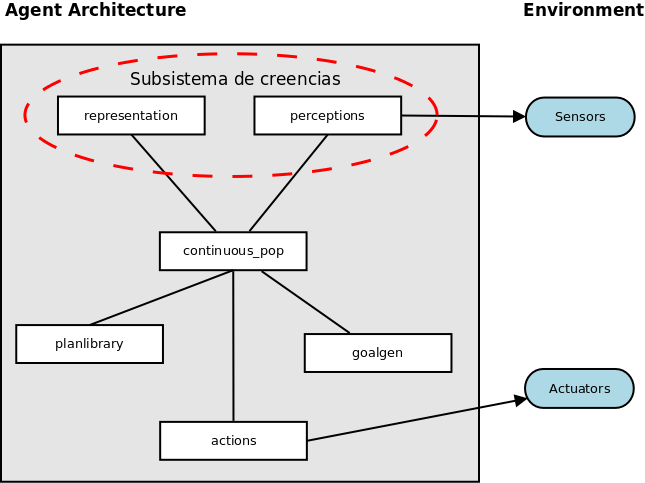
\includegraphics[width=9cm,height=8cm]{arqframework_BDI.png}
		\caption{El subsistema de creencias en la
	Arquitectura Modular del Framework.}
		\label{framework:modulesBDI}
	\end{figure}

Vemos que existen dos m\'odulos que dependen de una especificaci\'on STRIPS,
el m\'odulo \texttt{representation}, que contiene las acciones que el agente
puede ejecutar y el m\'odulo \texttt{perceptions}, que recibe percepciones
desde los sensores y las traduce a un representaci\'on STRIPS. Por lo
tanto, debido a que ambos m\'odulos constituyen el subsistema de
creencias del agente, tendremos un subsitema puramente especificado en PDDL.

En la figura \ref{framework:moduleswithPDDL}, podemos ver que 
los m\'odulos \texttt{perceptions} y \texttt{representation} 
dependen del traductor PDDL. Las percepciones
recibidas desde los sensores y la representaci\'on de las acciones del agente
son, entonces, traducidas a STRIPS. La l\'inea punteada en el gr\'afico
indica que ambos m\'odulos del subsistema de creencias dependen
de nuestro traductor.

% Ejemplo de una accion futbol en STRIPS y una en PDDL.

	\begin{figure}[h!]
	\centering
		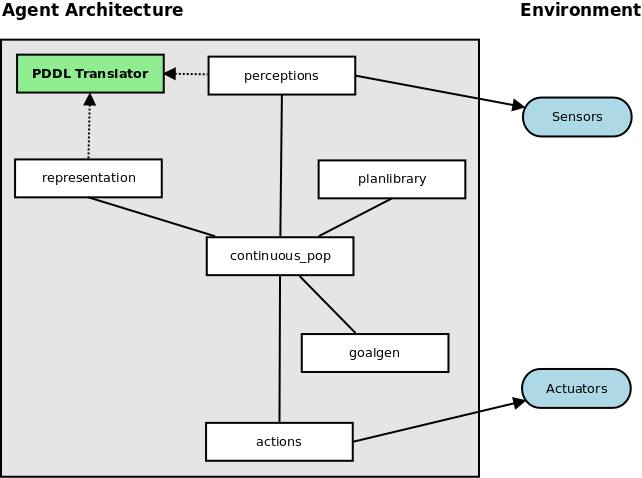
\includegraphics[width=8cm,height=7cm]{arqframework.png}
		\caption{Arquitectura del Framework y Traductor PDDL}
		\label{framework:moduleswithPDDL}
	\end{figure}


A continuaci\'on, mostramos un ejemplo de c\'omo especificamos
acciones del agente en PDDL. Primero, mostramos
la especificaci\'on de la acci\'on en STRIPS y luego,
la equivalente en PDDL. Por simplicidad, empleamos el mismo ejemplo utilizado
por Moya en \cite{gbraun:tesisMarioMoya}. 

\begin{ejemplo}%{Acciones del Agente en STRIPS}

En la acci\'on \texttt{move(Ag, Pos1, Pos2)}, el agente 
\texttt{Ag}, se desplaza de la posici\'on \texttt{pos1}
a la posici\'on \texttt{pos2}. 

 \begin{verbatim}
preconditions(move(Ag,Pos1,Pos2), [player(Ag),waiting_at(Ag,Pos1),
valid_move(Pos1,Pos2)]).
achieves(move(Ag,Pos1,Pos2),waiting_at(Ag,Pos2)).
deletes(move(Ag,Pos1,Pos2),waiting_at(Ag,Pos1)).
 \end{verbatim}
\end{ejemplo}

\begin{ejemplo}

La acci\'on equivalente en PDDL es la siguiente:

 \begin{verbatim}
(:action move
        (:parameters (?Ag ?Pos1 ?Pos2)
        (:precondition (and (player ?Ag) (waiting_at ?Ag ?Pos1)
                                         (valid_move ?Pos1 ?Pos2)))
        (:effect (and (waiting_at ?Ag ?Pos2) 
                      (not (waiting_at ?Ag ?Pos1))))
)        
 \end{verbatim}
\end{ejemplo}

El m\'odulo \texttt{perceptions} recibe el estado actual que incluye,
para el caso del F\'utbol de Robots, las coordenadas \texttt{X} e \text{Y} de los jugadores
y de la pelota. El siguiente ejemplo especifica el estado actual
usando PDDL.

\begin{ejemplo}%{Problema de f\'utbol de robots en PDDL}

Suponemos que el dominio de F\'utbol de Robots es llamado
\texttt{soccer\_domain} y los jugadores son nombrados
como \texttt{Ag} seguido de un n\'umero que lo identifica
un\'ivocamente en el problema. La meta es que el jugador
\texttt{Ag1} se desplace hacia la pelota \texttt{ball}.

 \begin{verbatim}
(define (problem soccer_problem)
(:domain soccer_domain)
(:objects Ag1 Ag2 Ag3 ball)
(:goal (carrying Ag1 ball))
(:init (at Ag1 cell1)
       (at Ag2 cell2)
       (at Ag3 cell3)
       (at ball cell4)
       (clear cell5)
       (clear cell6)
       (clear cell7))
)
 \end{verbatim}
\end{ejemplo}

Por lo tanto, proyectamos un planificador continuo cuyo lenguaje
de representaci\'on es PDDL.
\ \\

Hasta aqu\'i, hemos estudiado el lenguaje PDDL, la
implementaci\'on del Framework de Planificaci\'on Continua
desarrollado por Moya y vimos como el traductor PDDL propuesto
puede ser integrado al Framework.
En el cap\'itulo siguiente, analizaremos alternativas existentes y, a
partir del cap\'itulo \ref{pagcap6}, comenzaremos a delinear
nuestra implementaci\'on.


